\documentclass[10pt,a4paper]{article}
\usepackage{amsmath}
\usepackage{amssymb}
\usepackage{graphicx}
\usepackage{color}
\usepackage{fancyhdr}
\usepackage{fancyvrb}
\usepackage[margin=3.5cm]{geometry}
\usepackage{framed}
\usepackage{enumerate}
\usepackage{textcomp}
\def\ket#1{\left|#1\right\rangle}
\def\bra#1{\left\langle#1\right|}
\def\braket#1{\left\langle#1\right\rangle}

\definecolor{linkcol}{rgb}{0.0, 0.0, 0.7}
\usepackage[colorlinks=true,urlcolor=linkcol,citecolor=black,linkcolor=linkcol]{hyperref}

\renewcommand{\theequation}{1.\arabic{equation}}

\setcounter{section}{1}
\renewcommand\thesection{\arabic{section}}
\renewcommand\thesubsection{\thesection.\arabic{subsection}}

\fancyhf{}
\lhead{\tiny Y.~D.~Chong (2021)}
\rhead{\scriptsize MH2801: Complex Methods for the Sciences}
\lfoot{}
\rfoot{\thepage}
\pagestyle{fancy}

\begin{document}

\noindent
{\Large \textbf{1. Mathematical Functions}}
\vskip 0.2in

\label{mathematical-functions}

This is a course on complex methods in the physical sciences. But
before launching into a discussion on complex numbers, let us
undertake a brief review of real mathematical functions.

\subsection{Real functions}\label{real-functions}

A mathematical function, denoted $f$, takes an \textbf{input} $x$
(also called an \textbf{argument}), and returns an \textbf{output}
$f(x)$. For now, we consider the case where both $x$ and $f(x)$ are
real numbers. The set of possible inputs is the function's
\textbf{domain}, and the set of possible outputs is the
\textbf{range}.

Every function must have a well-defined output: for any $x$ in the
domain, $f(x)$ must be a specific, unambiguous number. In other words,
a function must be either a one-to-one (injective) map or a
many-to-one map; it cannot be one-to-many or many-to-many:

\begin{figure}[ht]
  \centering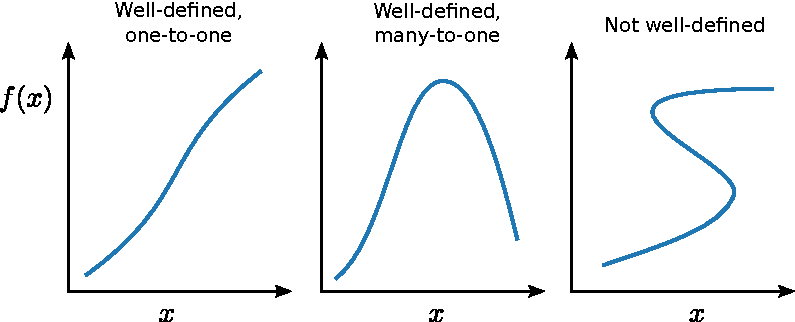
\includegraphics[width=0.8\textwidth]{mathfunctions}
\end{figure}

Simple examples of functions are those based on elementary algebra
operations:

\begin{align*}
  f(x) &= x + 2 \;\;\qquad \text{(a one-to-one function)} \\
  f(x) &= x^2 \quad\qquad \text{(a many-to-one function)}
\end{align*}

\subsection{The exponential function}
\label{exponential_function}

The exponential function, denoted by ``$\exp$'', is one of the most
important functions in mathematics. We will deal with it frequently,
in many different contexts.

It is very closely tied to the concept of power operations. Let us
start by examining what it means to take a number $x$ to the power of
$y$:
\begin{equation}
  f(x) = x^y.
\end{equation}
For values of $y$ in the natural numbers $\mathbb{N} \equiv
\{1,2,3,\dots\}$, the power operation simply means multiplying $x$ by
itself $y$ times.  For example, $x^4 = x \cdot x \cdot x \cdot x$.
But what about non natural number powers, like $x^{-1}$ or $x^{1/2}$
or $x^{\pi}$? As we shall see, the exponential will help us answer
this question.

We define the exponential function as the following limiting infinite series:
\begin{equation}
  \exp(x) \equiv 1 + \sum_{n=1}^\infty\frac{x^n}{n!}, \quad\mathrm{for}\;\, x \in \mathbb{R}.
  \label{eq:exp}
\end{equation}
(Note: the ``$\equiv$'' symbol is used to indicate a definition.)

Note that the infinite series in Eq.~\eqref{eq:exp} uses natural
number powers only.  The domain of this function is the set of real
numbers, $\mathbb{R}$, and its range is the set of positive numbers,
$\mathbb{R}^+$.

\clearpage
Here is a graph of the exponential function:

\begin{figure}[ht]
  \centering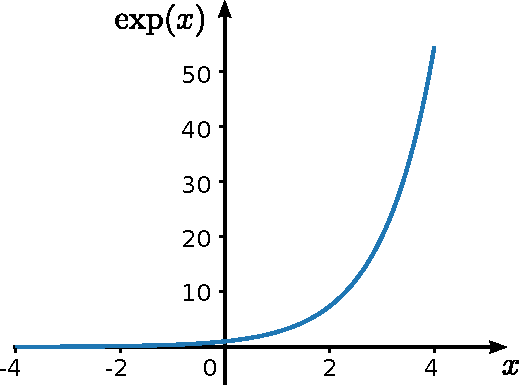
\includegraphics[width=0.4\textwidth]{exponential}
\end{figure}

\label{exponential-properties}

From this, we see that $\exp(x)$ increases \textit{very} quickly with
increasing $x$.  Going in the other direction, as $x$ decreases the
value of $\exp(x)$ approaches zero rapidly.

Moreover,
\begin{enumerate}
\item $\exp(0) = 1$. (This follows from the definition of the exponential.)

\item For all $x, y \in \mathbb{R}$,
  \begin{equation}
    \exp(x+y) = \exp(x)\,\exp(y)
    \label{eq:exponential_add}
  \end{equation}
  Try proving this as an exercise (see Section \ref{exercises}). The
  key ingredients for the proof are (i) the above definition of the
  exponential and (ii) the binomial theorem.

\item As a corollary of properties 1 and 2,
  \begin{equation}
    \exp(-x) = 1/\exp(x).
  \end{equation}
\end{enumerate}

\subsection{The logarithm function}
\label{the-logarithm-function}

Since the exponential is a one-to-one function, its inverse is a
well-defined function.  We call this the \textbf{natural logarithm}:
\begin{align}
  \ln(x) \equiv y \;\; \mathrm{such}~\mathrm{that}\; \exp(y) = x.
\end{align}
For brevity, we will use ``logarithm'' to refer to the natural
logarithm, unless otherwise stated; the ``non-natural'' logarithms are
not important in this course. From the definition of the logarithm, it
can be seen that the domain is $\mathbb{R}^+$ and the range is
$\mathbb{R}$ (the domain of the logarithm is the exponential's range,
and vice versa).  Its graph is shown below:

\begin{figure}[ht]
  \centering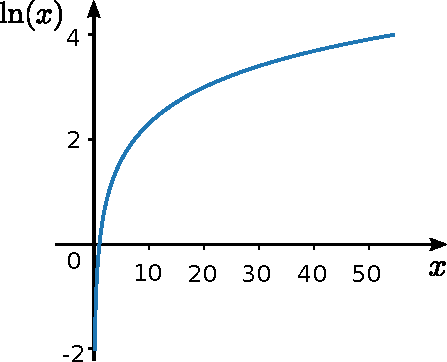
\includegraphics[width=0.4\textwidth]{logarithm}
\end{figure}

\noindent
Observe that $\ln(x)$ increases extremely slowly with $x$, which is
precisely the opposite of the exponential's behavior.

Using Eq.~\eqref{eq:exponential_add}, we can prove that the logarithm
satisfies the product and quotient rules
\begin{align}
  \ln(xy) &= \ln(x) + \ln(y) \\
  \ln\left(\frac{x}{y}\right) &= \ln(x) - \ln(y).
\end{align}

\subsection{Non-natural powers}
\label{powers}

Having defined the exponential and logarithm, we have the tools needed
to address the issue raised earlier, of how to define non-natural
powers.  First, observe that
\begin{align}
  \textrm{For}\;\,y \in \mathbb{N}, \;\;\;\ln(x^y) = \underbrace{\ln(x)\ln(x)\cdots\ln(x)}_{y\;\text{times}} = y \ln(x).
  \label{eq:lnxypower}
\end{align}
Hence, by applying the exponential to each side of
Eq.~\eqref{eq:lnxypower},
\begin{align}
  x^y = \exp[y \ln(x)] \quad \mathrm{for} \;\,y \in \mathbb{N}.
\end{align}
We can generalize the above equation so that it holds for any positive
$x$ and real $y$, not just $y \in \mathbb{N}$.  In other words, we
treat this as our \textit{definition} of the power operation for
non-natural powers:
\begin{align}
  x^y \equiv \exp[y \ln(x)] \quad\; \mathrm{when}\;\, x \in \mathbb{R}^+\;\textrm{and}\;y \notin \mathbb{N}.
\end{align}
By this definition, the power operation always gives a positive
result.  Moreover, for $y \in \mathbb{N}$, the formula is consistent
with the definition based on multiplying $x$ by itself $y$ times.

This generalization of the power operation leads to several important
consequences:
\begin{enumerate}
\item $\displaystyle x^0 = 1 \;\;\mathrm{for}\;\, x \in \mathbb{R}^+.$

\item Negative powers are reciprocals:
  \begin{align}
    x^{-y} = \exp[-y\ln(x)] = \exp[-\ln(x^y)] = \frac{1}{x^y}.
  \end{align}

\item The output of the exponential function is equivalent to a power
  operation:
  \begin{align}
    \displaystyle\exp(y) = e^y\quad\mathrm{where}\;\, e \equiv \exp(1) = 2.718281828459\!\dots
  \end{align}
  (This follows by plugging in $x=e$ and using the fact that $\ln(e) = 1$.)

\item For $x \le 0$, the meaning of $x^y$ for non-natural $y$ is
  ill-defined, since the logarithm does not accept negative
  inputs. (Later, we will see how this limitation can be bypassed.)
\end{enumerate}

\subsection{Trigonometric functions}
\label{trigonometric-functions}

Another extremely important group of functions are the fundamental
trignonometric functions $\sin$, $\cos$, and $\tan$.  These can be
defined in terms of the geometric ratios of the sides of right-angled
triangles, as shown below:

\begin{figure}[h!]
  \centering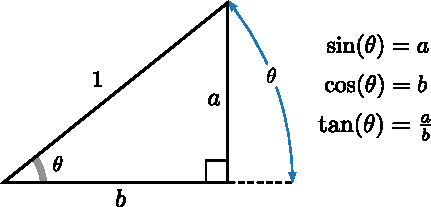
\includegraphics[width=0.4\textwidth]{trigonometry}
\end{figure}

\clearpage

\noindent
If we use this basic definition, the domain is $\theta \in [0,
  \,\pi/2)$, where the input angle $\theta$ is given in radians.

We can generalize the definition using the following scheme, which
allows for negative values of $a$ and/or $b$:

\begin{figure}[h!]
  \centering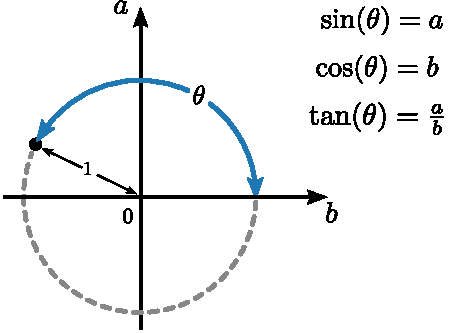
\includegraphics[width=0.4\textwidth]{trigonometry2}
\end{figure}

\noindent
With this, the domain is extended to $\theta \in [0,\,2\pi)$. We can
  further extend the domain to all real numbers, $\theta \in
  \mathbb{R}$, by treating input values modulo $2\pi$ as equivalent,
  i.e., $f(\theta + 2\pi) = f(\theta)$.  Then the trigonometric
  functions become many-to-one functions.

According to the \href{http://www.faculty.umb.edu/gary_zabel/Courses/Phil%20281b/Philosophy%20of%20Magic/Arcana/Neoplatonism/Pythagoras/index.shtml.html}{Pythagorean theorem},
\begin{align}
  \big[\sin(\theta)\big]^2 + \big[\cos(\theta)\big]^2 = 1.
\end{align}
Using this, we can go on to prove a variety of identities, like the
addition identities
\begin{align}
  \sin(\theta_1 + \theta_2) &= \sin(\theta_1) \cos(\theta_2) + \cos(\theta_1)\sin(\theta_2) \\
  \cos(\theta_1 + \theta_2) &= \cos(\theta_1) \cos(\theta_2) - \sin(\theta_1)\sin(\theta_2).
\end{align}
As you may recall, the trigonometric proofs for these identities
involve drawing complicated triangle diagrams, cleverly applying the
Pythagorean formula, and other tricks.  There are two problems with
such geometrical proofs: (i) they require some ingenuity in the
construction of the triangle diagrams, and (ii) it may not be obvious
whether the proofs work if the angles lie outside
$[0,\pi/2)$. Happily, there is a solution to both problems. As we
  shall see, trigonometric identities can be proven algebraically with
  complex numbers.

\subsection{Hyperbolic functions}\label{hyperbolic-functions}

The hyperbolic functions are important functions defined in terms of
exponentials:
\begin{align}
  \sinh(x) &= \frac{1}{2}\left(e^{x} - e^{-x}\right) \\
  \cosh(x) &= \frac{1}{2}\left(e^{x} + e^{-x}\right) \\
  \tanh(x) &= \frac{e^{x} - e^{-x}}{e^{x} + e^{-x}}.
\end{align}
They have properties that are intriguingly similar to the trignometric
functions. For example,
\begin{align}
  \sinh(x+y) &= \sinh(x)\cosh(y) + \cosh(x)\sinh(y) \\
  \cosh(x+y) &= \cosh(x)\cosh(y) + \sinh(x)\sinh(y)
\end{align}
Because of these identities, it is sometimes more convenient to work
with hyperbolic functions rather than exponentials. As we shall see,
there is an intricate relationship between the hyperbolic and
trigonometric functions.

\subsection{Continuity (optional topic)}

\textbf{Continuity} is an important concept in the theory of real
functions. A continuous function is one whose output $f(x)$ does not
undergo abrupt jumps when $x$ changes by tiny amounts.  A function can
be continuous over its entire domain, or only a subset of its
domain. For example, $\sin(x)$ is continuous for all $x$, whereas
$f(x) = 1/x$ is discontinuous at $x = 0$.  Another function that is
discontinuous at $x=0$ is the step function
\begin{align}
  \Theta(x) = \left\{\begin{array}{ll} 1, &\;\;\;\textrm{for} \; x \ge 0\\ 0,&\;\;\; \textrm{otherwise.}\end{array}\right.
\end{align}
Mathematicians have even come up with functions that are discontinuous
everywhere in their domain, but we won't deal with such things.

The rigorous definition of continuity is as follows:
\begin{framed}
\noindent
  A function $f$ is continuous at a point $x_0$ if, for any $\epsilon >
0$, we can find a $\delta > 0$ such that setting $x$ closer to $x_0$
than a distance of $\delta$ brings $f(x)$ closer to $f(x_0)$ than the
specified distance $\epsilon$.
\end{framed}

\noindent
That's a pretty complicated sentence! The plot below may help you to
understand it:

\begin{figure}[ht]
  \centering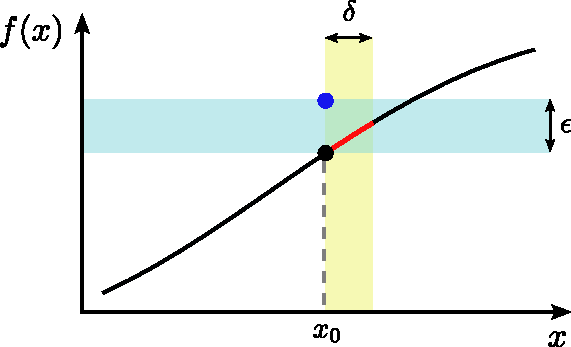
\includegraphics[width=0.45\textwidth]{continuity}
\end{figure}

\noindent
At the selected point $x_0$, the value $f(x_0)$ is indicated by the
black dot.  Now, for a given choice of epsilon, $f(x_0)+\epsilon$ is
indicated by the blue dot.  One can choose $\delta$ so that for all
$x_0 < x < x_0 + \delta$ (the region shaded in yellow), $f(x)$ is
closer to $f(x_0)$ than the blue dot.

A counter-example, with a function that has a discontinuity at some
$x_0$, is shown below:

\begin{figure}[ht]
  \centering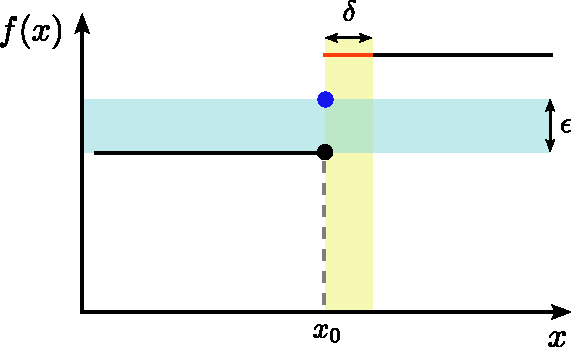
\includegraphics[width=0.45\textwidth]{discontinuity}
\end{figure}

\noindent
If we choose $\epsilon$ smaller than the gap, then no matter what
value of $\delta > 0$ we try, any choice of $0 < x < \delta$ will give
a value of $f(x)$ further than $\epsilon$ from $f(x_0)$. Hence, the
continuity condition is violated for sufficiently small choices of
$\epsilon$, and $f$ is \textbf{discontinuous} at $x_0$.

\subsection{Exercises}\label{exercises}

\begin{enumerate}
  \def\labelenumi{\arabic{enumi}.}
\item
  An alternative definition of the exponential function is the limiting
  expression
  \begin{equation}
    \exp(x) \equiv \lim_{n\rightarrow\infty} \left(1+\frac{x}{n}\right)^n.
  \end{equation}
  Prove that this is equivalent to the definition in terms of an
  infinite series,
  \begin{equation}
    \exp(x) \equiv 1 + \sum_{n=1}^\infty\frac{x^n}{n!}.
  \end{equation}

\item
  Prove that
  \begin{equation}
    \exp(x+y) = \exp(x)\,\exp(y)
  \end{equation}
  using the definition of the exponential as an infinite series. Your
  proof must avoid using the concept of ``raising to the power'' of a
  non-natural number; this is to avoid circular logic, since this
  feature of the exponential function can be used in the generalized
  definition of the power operation (Section \ref{powers}).
  \hfill{\scriptsize [solution~available]}

\item
  One of the most important features of the exponential function
  $\exp(x)$ is that it becomes large \emph{extremely} quickly with
  increasing $x$. To illustrate this behavior, consider the graph
  shown in Section~\ref{exponential_function}, which plots the
  exponential up to $x = 4$.  On your screen or page, the height of
  the graph should be around 4 cm. Suppose we keep to the same
  resolution, and plot up to $x = 10$; how high would the graph be?
  What if we plot up to $x = 20$?

\item
  Prove that $\displaystyle \exp(x) = e^x.$
  \hfill{\scriptsize [solution~available]}

\item
  A ``non-natural'' logarithm of base $c$ is defined as
  \begin{equation}
    \log_c(x) = y \quad\mathrm{where}\;\; c^y = x.
  \end{equation}
  Derive an expression for the non-natural logarithm in terms of the
  natural logarithm.

\item
  Prove, using trigonometry, that
  \begin{equation}
    \sin(\theta_1 + \theta_2) = \sin(\theta_1) \cos(\theta_2) + \cos(\theta_1)\sin(\theta_2).
  \end{equation}
  You may assume that $\theta_1, \theta_2 \in [0, \pi/2].$

\item
  Prove that
  \begin{align}
    \cos(3x) &= 4[\cos(x)]^3 -3\cos(x) \\
    \sin(3x) &= 3\sin(x)-4[\sin(x)]^3.
  \end{align}
\end{enumerate}

\end{document}
